%\documentclass{beamer}
\documentclass[handout]{beamer}

\usepackage{pgfpages} 

%\setbeameroption{show only notes}

\usetheme{default}

\mode<presentation> {
%  \usetheme{Warsaw}
  \usetheme{Frankfurt}
%  \usetheme{Boadilla}
%  \usetheme{Marburg}
}

\mode<handout>{\setbeamercolor{background canvas}{bg=black!5} %
    \pgfpagesuselayout{4 on 1}[letterpaper,border shrink=4mm,landscape] %
    \setbeameroption{show notes}}

\title[CAC Overview] {CAC Overview}
\author{Brock Palen\\ \texttt{brockp@umich.edu}}
\date{TBD}

\begin{document}
  \setbeamercovered{transparent}  
  \begin{frame}
    \titlepage
    \url{http://cac.engin.umich.edu/training}
  \end{frame}

%table of contents
  \begin{frame}{Outline}
    \tableofcontents
  \end{frame}
  
  \section {Hardware}
   \subsection{Compute}
    \begin{frame}{Compute}
     \begin{block}{Compute}
      \begin{itemize}
       \item{3100+ x86\_64 CPU's Grows Monthly}
       \item{32 Itanium II's}
       \item{2GB Memory/CPU 5532GB Ram total (2/9/2009)}
       \item{Upto 96/64GB Memory to single thread}
      \end{itemize}
     \end{block}
     \begin{block}{Non Standard Compute}
      \begin{itemize}
       \item<2->{GPGPU's}
       \item<2->{40 Total GPU's}
      \end{itemize}
     \end{block}
    \end{frame}
    \begin{frame}{Pre/Post Processing}
      \begin{center}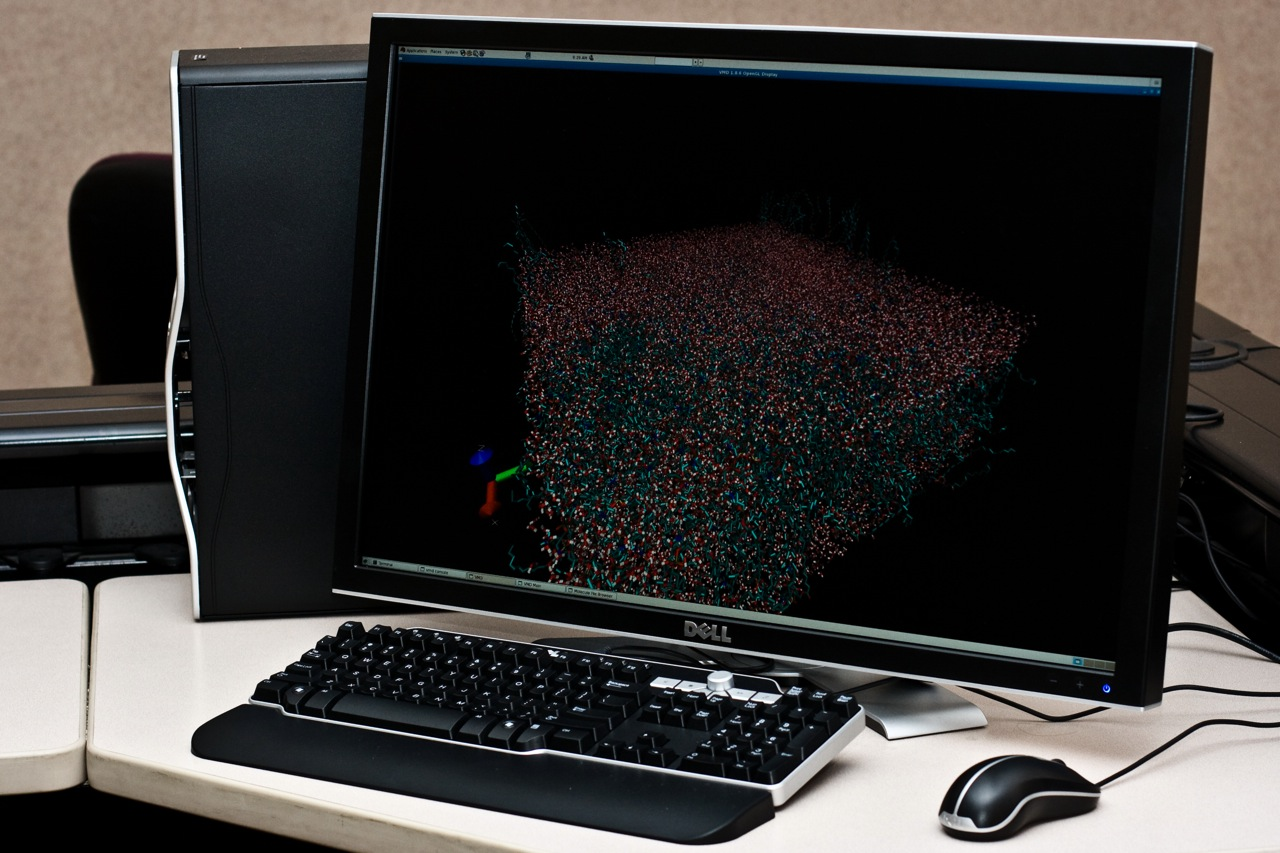
\includegraphics[height=2.0in]{3dlab}\end{center}
      \begin{block}{Hardware/Software}
       \begin{itemize}
         \item Full CAEN Linux Load
         \item 2 Systems, 16GB, Quatro GPU, very big screen
       \end{itemize}
      \end{block}
    \end{frame}
   \subsection{Networks}
    \begin{frame}{Networks}
     \begin{block}{Networks}
      \begin{itemize}
       \item Every node has 1Gbps Ethernet full nonblocking
       \item 98+ Nodes with 20Gbps Infiniband
       \item Over 2 Tbps network ability
       \item 10Gbps link to North Campus
      \end{itemize}
     \end{block}
    \end{frame}
   \subsection{Storage}
    \begin{frame}{Storage}
     \begin{block}{Comodity Storage}
      \begin{itemize}
       \item \texttt{/home/} 40GB Quota available by NFS, snapshots no backups
       \item \texttt{/afs/} AFS Tokens for \texttt{umich.edu} cell on login, any token allowed on login nodes
      \end{itemize}
     \end{block}
     \begin{block}{Performance Storage}
      \begin{itemize}
        \item \texttt{/nobackup/} 50TB Parallel filesystem
        \item Supports writes upto 700MB/s Reads 650MB/s
        \item Supports MPI-IO and other Parallel IO
        \item Mounted on \texttt{login.engin.umich.edu}
        \item Mounted on 3D Lab Linux Machines
      \end{itemize}
     \end{block}
    \end{frame}
  \section {Training}
     \begin{frame}{Training}
      \begin{block}{Training}
       \begin{itemize}
        \item CAC Provides Introduction training on use of PBS and Resources
        \item Supliment Topics are added as requested
        \begin{itemize}
         \item Introduction to MPI Parallel Programming
         \item BLAS/LAPACK High Performance Mathematics
         \item User Round Tables (Matlab so far)
        \end{itemize}
        \item Offered 3 times a year
        \item Offered on demand for groups of users (new or not)
       \end{itemize}
      \end{block}
      \url{http://cac.engin.umich.edu/training/}
     \end{frame}
  \section {Software}
    \subsection {Development Tools}
     \begin{frame}{Development Software}
      \begin{block}{Tools}
       \begin{itemize}
         \item PGI/Intel/Nag Compilers
         \item GNU Compilers (not recomended)
         \item Code Profilers, Serial and Parallel (opt)
         \item Debuggers, Serial and Parallel (ddt)
         \item Code Coverage Analysis 
       \end{itemize}
      \end{block}
     \end{frame}
     \begin{frame}{Debelopment Software}
      \begin{block}{Libraries}
        \begin{itemize}
         \item MPI Parallel Libraries that support multiple network types
         \item NAG/IMSL High Level Math Libraries, Serial and Parallel
         \item BLAS/LAPACK Parallel Linear Algerbra Software
         \item Sparse Matrix Solvers (Pardiso, MKL, etc)
         \item CPLEX Optimization LP Problems
         \item Any CAEN Library, is a CAC Library
        \end{itemize}
      \end{block}
     \end{frame}
    \subsection{Applications}
     \begin{frame}{Applications}
      \begin{block}{Applications}
       \begin{itemize}
        \item CAC Works with CAEN (On Demand) for ISV applications
        \begin{itemize}
          \item Matlab/Minos/Fluent/Abaqus/etc.
        \end{itemize}
        \item We build and install common used applications
        \begin{itemize}
          \item R/Amber/AutoDock/Lammps
        \end{itemize}
        \item CAC supports faculty owned software installations, and control access to application
       \end{itemize}
      \end{block}
      \url{http://cac.engin.umich.edu/resources/systems/nyxV2/software.html}
     \end{frame}
  \section{Examples}
\end{document}
